\documentclass[10pt, reqno, letterpaper, twoside]{amsart}
\usepackage[margin=1in]{geometry}

\usepackage{amssymb, bm, mathtools}
\usepackage[usenames,dvipsnames,svgnames,table]{xcolor}
\usepackage[pdftex, xetex]{graphicx}
\usepackage{enumerate, setspace}
\usepackage{float, colortbl, tabularx, longtable, multirow, subcaption, environ, wrapfig, textcomp, booktabs}
\usepackage{pgf, tikz, framed, url, hyperref}
\usepackage[normalem]{ulem}
\usetikzlibrary{arrows,positioning,automata,shadows,fit,shapes}
\usepackage[english]{babel}

\usepackage{microtype}
\microtypecontext{spacing=nonfrench}

\usepackage{times}
\title{Indoor-Outdoor Localization for Ground Robots using Factor Graphs}
\author{
Evan Grant [edgrant@seas],
Rithwik Udayagiri [rithwiku@seas],
Aadith Kumar [aadith@seas],
}

\begin{document}

% \input{instructions}

\begin{abstract}

This project implements algorithms for autonomous navigation on a real ground robot in an environment comprising both indoor and outdoor regions using 3D LiDAR, GPS, and odometry estimates. These algorithms involve Mapping, Localization, Control and Sensor Fusion using factor graphs and the GTSAM library. The challenge of localizing in hybrid indoor and outdoor maps is addressed with complementary sensing modalities: GPS which is only reliable outside and LiDAR which only performs robustly indoors.

Mapping, Localization, Control and Sensor Fusion algorithms make the bulk of this project to complete a loop which was demonstrated on a real robot - AgileX Scout 2.0 in and around Penn Engineering buildings.
\end{abstract}

\maketitle

\section{Introduction}

Localization plays a crucial role in enabling robots to navigate safely around obstacles and follow pre-planned trajectories. However, the techniques currently used in the industry are typically optimized for either indoor or outdoor settings. Consequently, algorithms and sensors designed for indoor localization often do not perform well in outdoor environments and vice versa.

To overcome this challenge, we are exploring the fusion of multiple sensor modalities and localization outputs to achieve robust positioning results for both indoor and outdoor spaces. This is essential for facilitating seamless robot navigation across different environments, which is becoming increasingly important with the growing flexibility of robot designs for indoor and outdoor use.

Indoor-outdoor localization has numerous practical use cases, such as robots that can navigate through a building and then move outside to a parking lot to complete a task, or robots that can traverse a warehouse and then navigate outside to a loading dock for a job. By addressing the challenge of localization in both indoor and outdoor environments, we can help enhance the versatility of robots and broaden their scope of applications.

In this project, we have used HDL Graph SLAM for mapping and localization, a Pure Pursuit controller for trajectory following, and a factor graph based sensor fusion algorithm to fuse GPS, odometry and LiDAR data. Purely LiDAR based localization with Pure Pursuit was tested on a AgileX Scout 2.0 robot. The sensor fusion algorithm was tested on a simulated dataset from real map waypoints and synthetic noise.


\subsection{Contributions}

% Add figure
\begin{figure}[h]
    \centering
    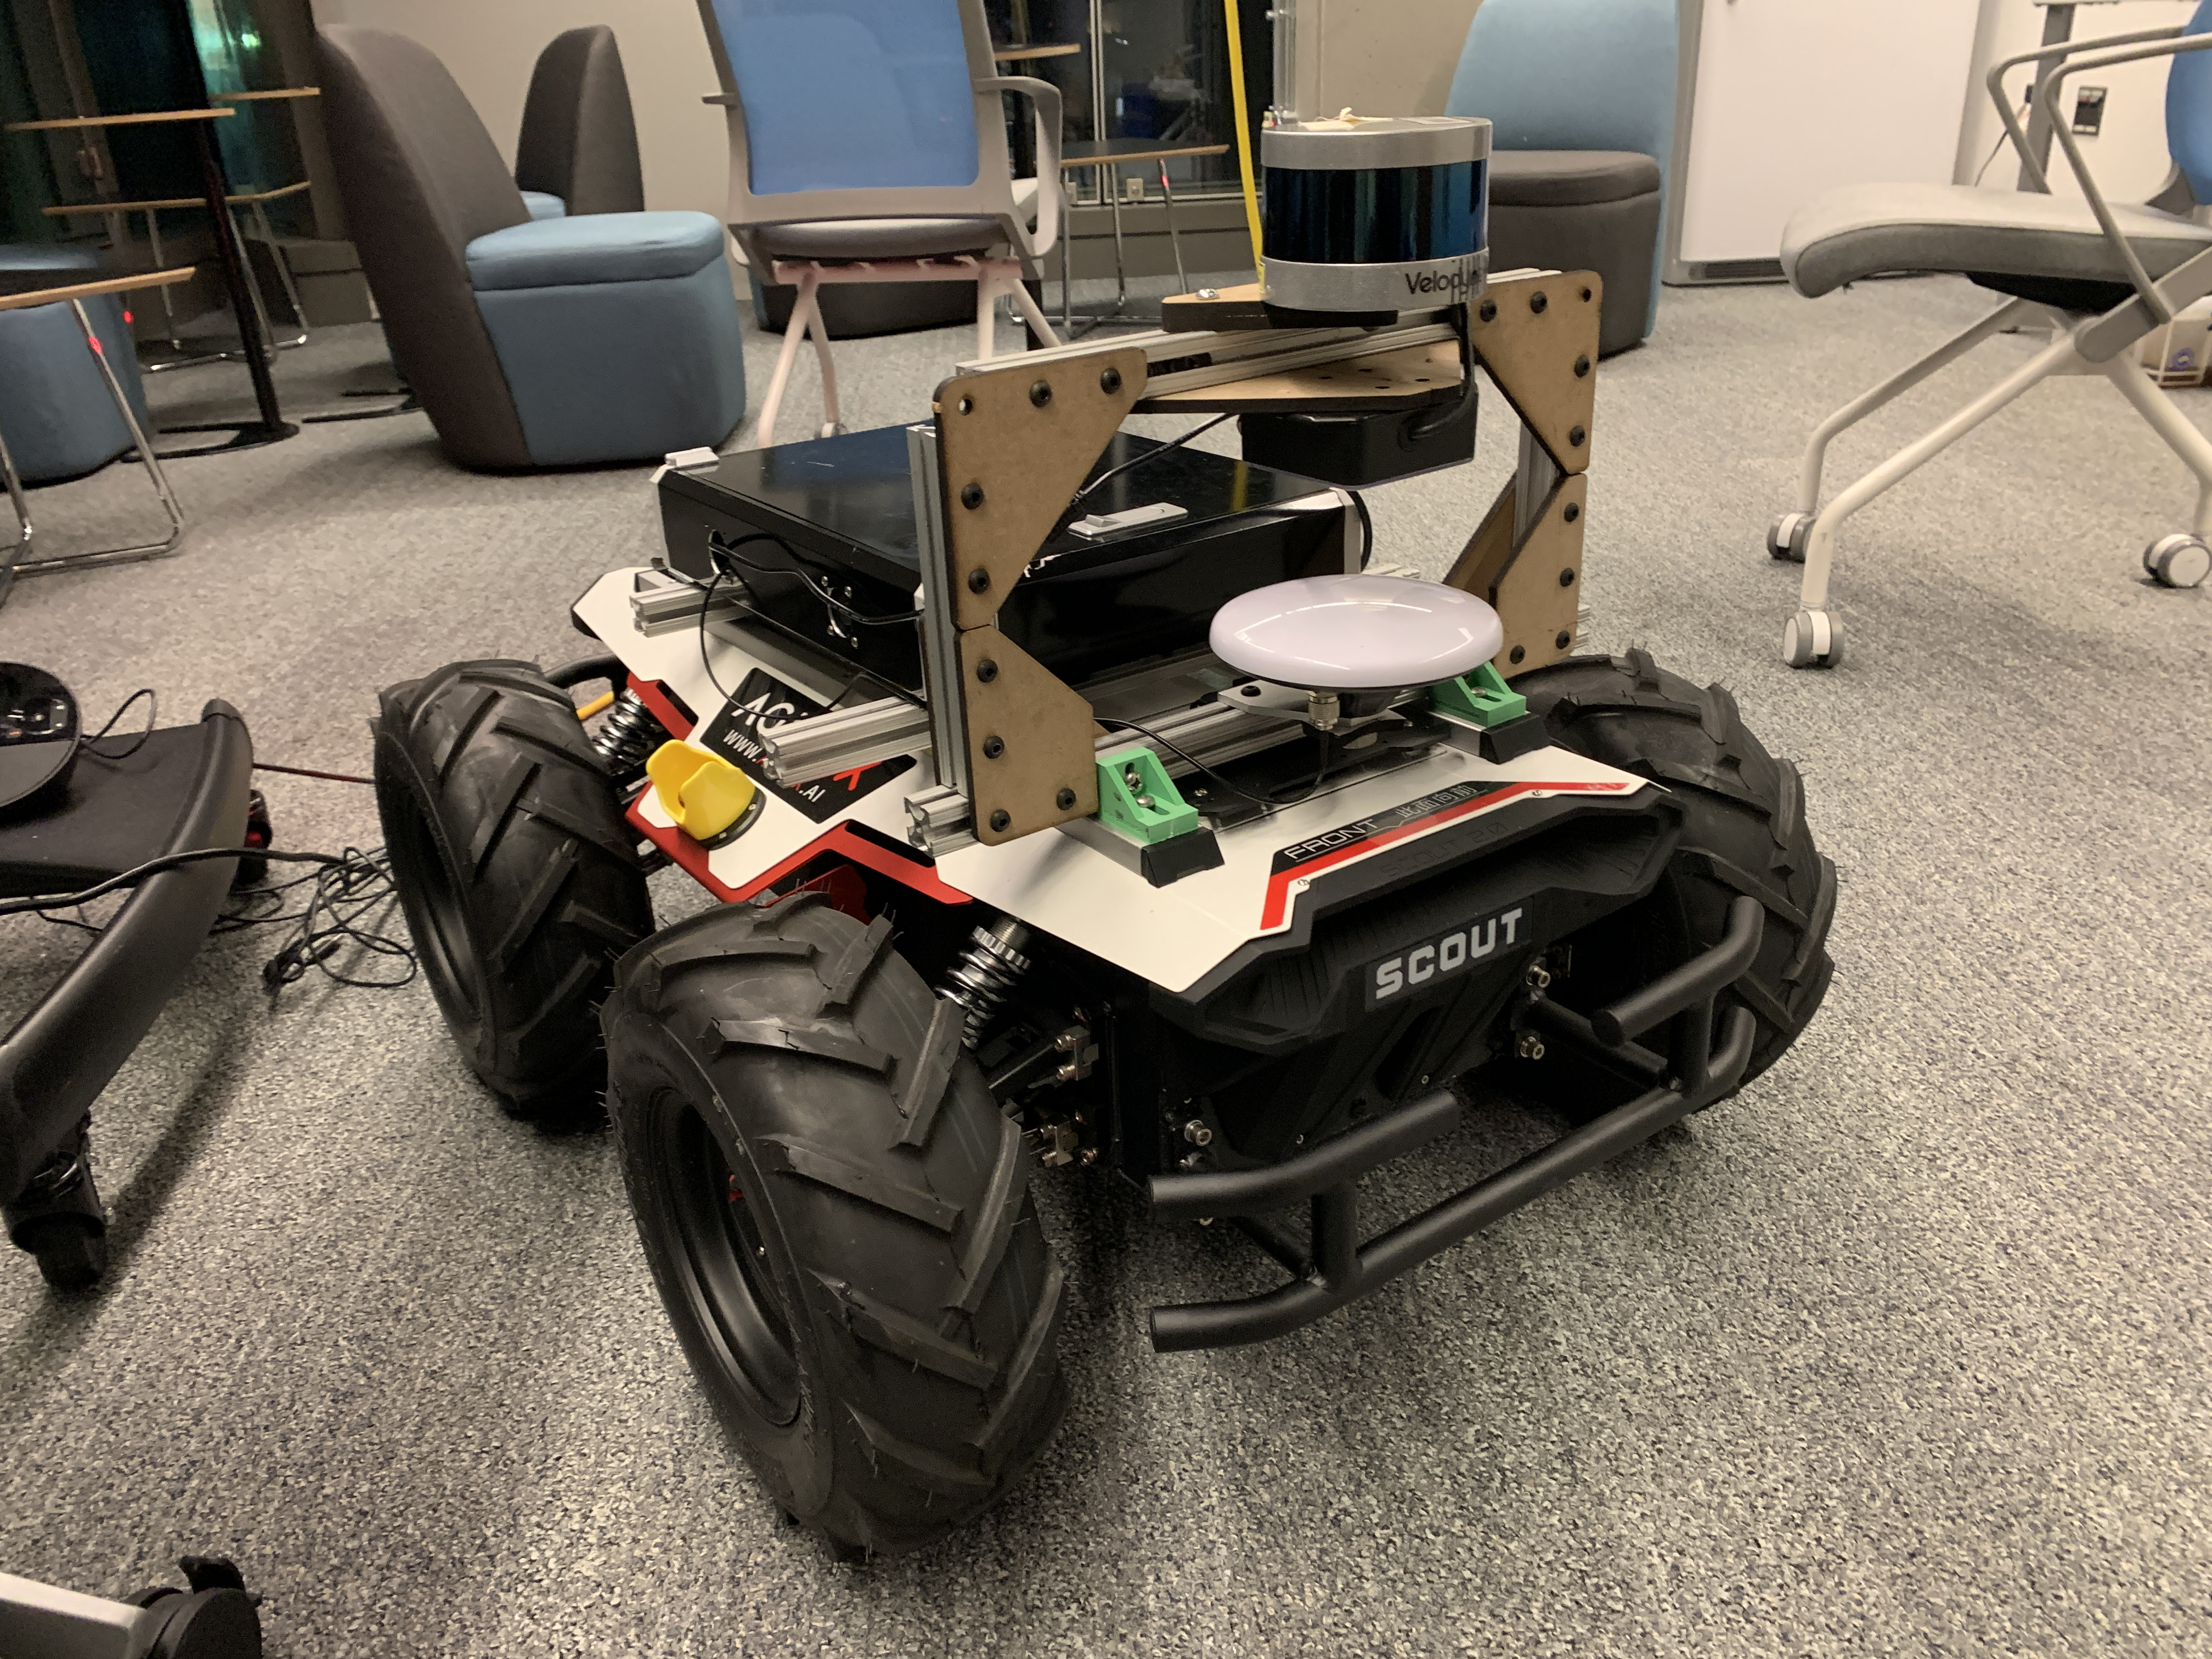
\includegraphics[width=0.5\textwidth]{figures/robot.png}
    \caption{AgileX Scout 2.0}
    \label{fig:robot}
\end{figure}

\begin{itemize}
    \item We implemented a factor graph based SLAM algorithm for mapping and localization.
    \item We implemented a control algorithm to follow a trajectory.
    \item We implemented a sensor fusion algorithm to fuse GPS, odometry and LiDAR data.
    \item We demonstrated the above algorithms on a real robot - AgileX Scout 2.0.

\end{itemize}

A list of concrete results in the report that the reader can quickly ascertain/understand.

\section{Background}

Introduce the problem and the notation if any.

\section{Related Work}

Note down references. Say how they relate to your approach. Your objective to put your work in context of the broader literature, namely, what other possible approaches exist for this problem, what they are good at or what they lack, what your approach does differently from them.

\section{Approach}

Details of your approach.

\section{Experimental Results}

Make sure you write clearly which datasets/architectures are used, how you pre-process the data, why you are reporting the metrics you are reporting. You should not simply say ``I did this experiment and this is the error'' like you'd do in a problem set. The objective of this section is to interpret the results, explain what they mean, what is good, what is bad etc.

\section{Discussion}

This section explains how to interpret the results in the context of the broader literature. You can talk about what did not work, what you'd like to do if you have more time/data/resources or more long-term investment that one would need to do to solve this specific problem.

\section{Acknowledgements}

We would like to extend our gratitude to those who enabled our work. Thanks to Dr. Nadia Figueroa for welcoming us into the lab space and for generously providing us with the AgileX Scout 2.0 platform. Thanks to Fernando Cladera for supplying us with the Velodyne LiDAR and all the hardware and firmware troubleshooting assistance thereafter. Finally, thanks to Dr. Pratik Chaudhari for his assistance with project formulation and providing insight regarding factor graph implementation and the GTSAM library.
% \section*{References}

\bibliographystyle{IEEEtran}
% Include bibliography file
\bibliography{IEEEabrv,references}

\end{document}